\section{Investigación}

\subsection{Giroscopio}
El giroscopio es un sensor que mide la velocidad angular en uno o más ejes, permitiendo detectar cambios en la orientación de un objeto. Este dispositivo es fundamental en aplicaciones que requieren estabilización y control de movimiento, como en cámaras, drones, sistemas de navegación inercial, videojuegos y dispositivos móviles \cite{MEMS}. Los giroscopios modernos, basados en tecnología MEMS (Micro-Electro-Mechanical Systems), son compactos, precisos y de bajo costo, lo que los hace ideales para su integración en sistemas robóticos y dispositivos portátiles.

En la \autoref{fig:giroscopio} se muestra un ejemplo de un giroscopio utilizado en aplicaciones de robótica y electrónica.

\begin{figure}[h]
	\centering
	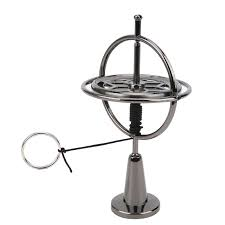
\includegraphics[width=0.3\linewidth]{img/Giroscopio}
	\caption{Ejemplo de un giroscopio utilizado en sistemas de navegación y estabilización.}
	\label{fig:giroscopio}
\end{figure}

\subsection{Acelerómetro}
El acelerómetro es un sensor que mide la aceleración lineal en uno o más ejes, permitiendo detectar movimientos, vibraciones e inclinaciones. Este dispositivo es ampliamente utilizado en teléfonos inteligentes, wearables, automóviles, drones y maquinaria industrial \cite{Acelerometro}. Los acelerómetros basados en tecnología MEMS son especialmente populares debido a su pequeño tamaño, bajo consumo de energía y alta precisión.

En la \autoref{fig:acelerometro} se muestra un ejemplo de un acelerómetro utilizado en aplicaciones de robótica y dispositivos móviles.

\begin{figure}[h]
	\centering
	\includegraphics[width=0.3\linewidth]{img/Acelerómetro}
	\caption{Ejemplo de un acelerómetro utilizado en sistemas de detección de movimiento.}
	\label{fig:acelerometro}
\end{figure}

\subsection{Magnetómetro}
El magnetómetro es un sensor que mide la intensidad y dirección de campos magnéticos, funcionando como una brújula digital. Este dispositivo es esencial en sistemas de navegación, donde se utiliza para determinar la orientación respecto al campo magnético terrestre. Además, los magnetómetros se emplean en aplicaciones de exploración geofísica, detección de metales y estudios de materiales magnéticos \cite{MEMS}.

En la \autoref{fig:magnetometro} se muestra un ejemplo de un magnetómetro utilizado en sistemas de navegación y exploración.

\begin{figure}[h]
	\centering
	\includegraphics[width=0.3\linewidth]{img/Magnetómetro}
	\caption{Ejemplo de un magnetómetro utilizado en sistemas de navegación y detección de campos magnéticos.}
	\label{fig:magnetometro}
\end{figure}

\subsection{LiDAR (Light Detection and Ranging)}
El LiDAR es una tecnología que mide distancias utilizando pulsos de luz láser, permitiendo generar mapas tridimensionales de alta precisión. Este sistema es ampliamente utilizado en vehículos autónomos para la detección de obstáculos y la navegación en entornos complejos. Además, el LiDAR se emplea en aplicaciones de cartografía, arqueología y estudios ambientales, donde es necesario obtener datos topográficos detallados \cite{LIDAR}.

En la \autoref{fig:lidar} se muestra un ejemplo de un sistema LiDAR utilizado en vehículos autónomos y aplicaciones de mapeo.

\begin{figure}[h]
	\centering
	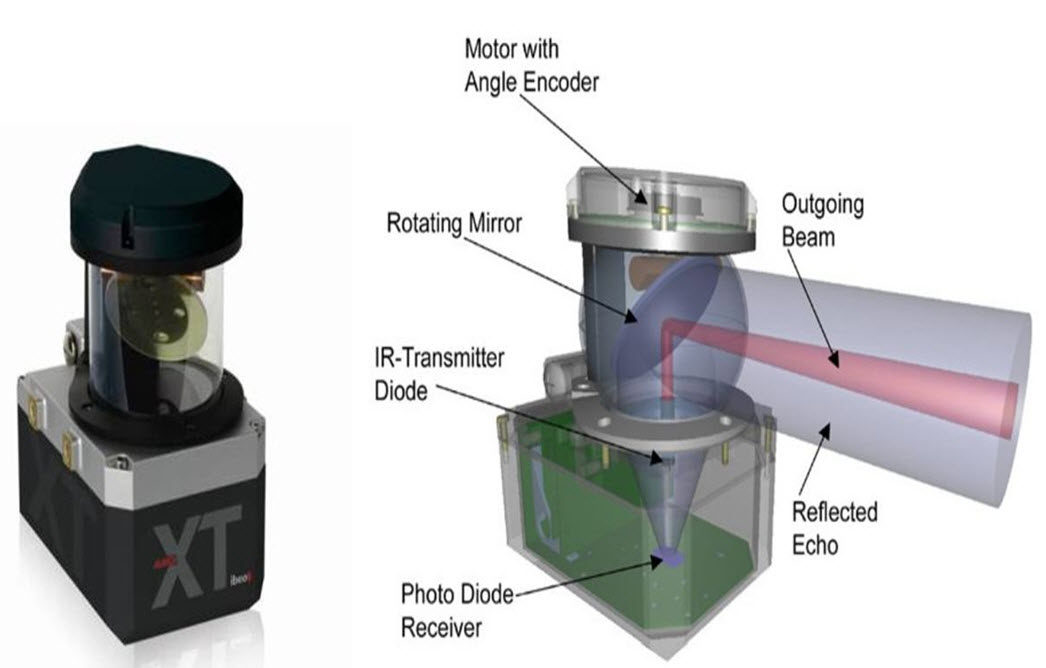
\includegraphics[width=0.5\linewidth]{img/LiDAR}
	\caption{Ejemplo de un sistema LiDAR utilizado en vehículos autónomos y cartografía.}
	\label{fig:lidar}
\end{figure}